% Chapitre sur le rapport d ingenierie :


\chapter{Rapport d'ingénierie} 


\TODO {ADD definitions to glossary !!!!}






\section*{Introduction}

Ce PFE conclut les cinq années d'étude a l'INSA de Lyon. 
Il s'agit de démontrer des capacités d'adaptation, d'innovation et d'initiative propres a un ingénieur. Les laboratoires aux 
États-Unis ont besoin de l'expertise d'ingénieurs pour résoudre des problème techniques. 
Notamment, au Megason Lab, ce sont principalement des ingénieurs qui développent le programme de visualisation de données. 
Les problèmes d'acquisitions d'images biologiques révèlent aussi des défis techniques.
 
\section*{Objectifs}

Les objectifs initialement proposés contenaient une très forte composante recherche.
Cependant, le Megason lab cherche au maximum a intégrer les avancées en traitement de l'image aux outils qu'il conçoit,
 notamment au programme Gofigure2. Cela entraine des contraintes vis à vis des outils de développements. 
 Il a donc fallu me former afin que je devienne un programmeur avancé en {\C++}. 
 
J'ai ainsi commencé mon PFE en tant que membre de l'équipe de développement de Gofigure2.
 Les objectifs étant d'apprendre les différentes librairies utilisées par le programme, pour mettre au point un système de plugins. 
 Ma mission était de créer une librairie de comparaison d'images, afin d'inclure aux plugins, un aperçu à la Photoshop.

Dans le cadre de ma participation au développement de Gofigure2,
 j'ai aussi proposé un protocole de travail avec un nouveau programme de contrôle de version : GIT.
 Il s'agissait tout d'abord d'apprendre à utiliser GIT, pour ensuite transmettre ce savoir et enfin proposer une méthode de travail.

Mon PFE étant motivé par des objectifs de traitement de l'image, j'ai aussi travaillé sur l'amélioration
 des techniques d'acquisitions de données microscopiques.





%--------------------------------------------------
%             COMPARAISON
%--------------------------------------------------


\section{Création d'une librairie de comparaison d'images}

L'équipe d'informaticiens au Megason Lab est divisée en deux : deux ingénieurs travaillent sous la direction d'un docteur sur la
 création de l'outil de visualisation d'images microscopiques (GoFigure2), tandis qu'un autre docteur travaille sur
 des algorithmes de traitement d'image. Afin de travailler pour l'ensemble des informaticiens, le projet devait
\begin{inparaenum}[(i)]
  \item faciliter le travail de développement d'algorithmes de traitement de l'image, et 
  \item s'intégrer au développement de GofiGure2.
\end{inparaenum}

La création de la librairie de comparaison d'images atteint ces deux buts : 
Il s'agit d'un programme utilisant le code source du projet Gofigure2, 
qui sera utilisé pour le développement des plugins de Gofigure2.
Cette librairie a enfin était spécifiquement développée pour compléter le projet de débugger graphique de 
Matt MacCormick \cite{McCornic-VisualDebug}, afin de rendre cette librairie particulièrement utile
aux traiteurs d'image développant sous ITK.
Ce programme permet aussi de visualiser les traitements appliques aux données
lors de l'exécution d'un algorithme de traitement d'image sous un environnement de debugging (gdb\TODO{definir GDB}).


\subsection{cahier des charges}


\begin{figure}[H]
\begin{center}
\leavevmode
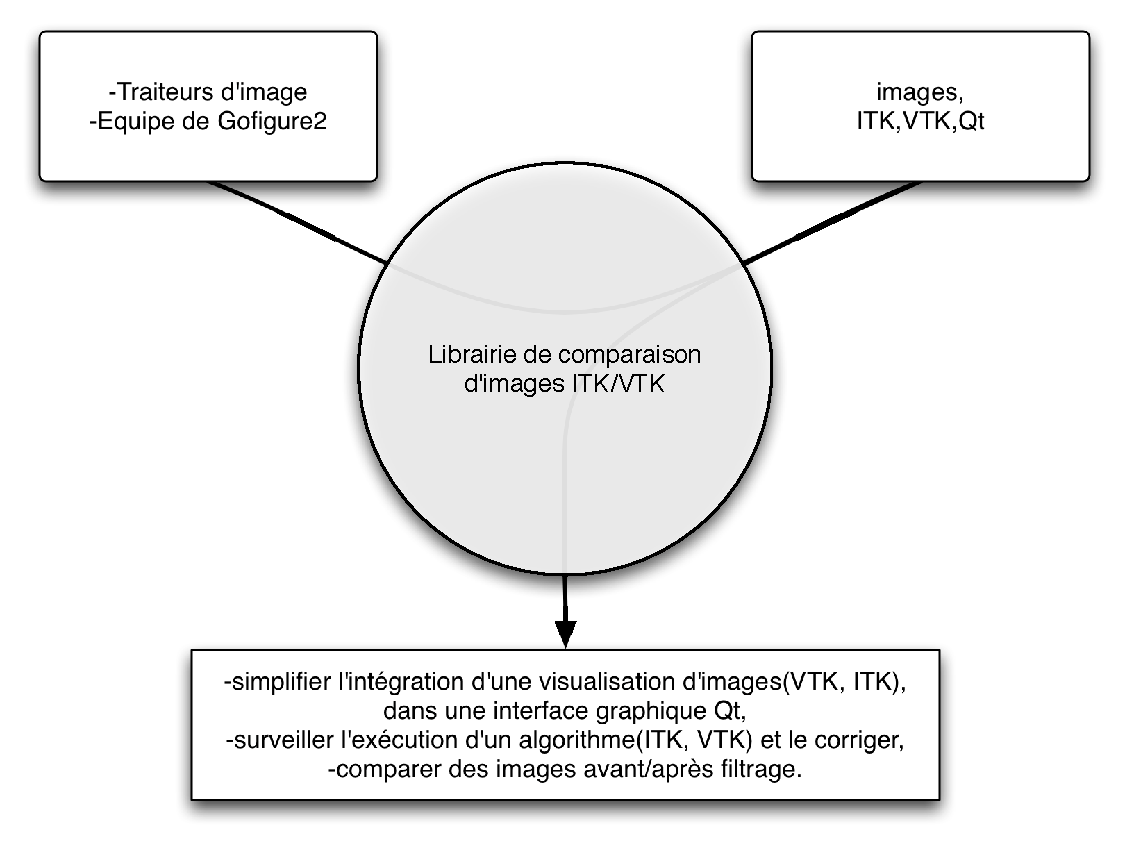
\includegraphics[width=0.95\textwidth]{pictures/CompareBAC}
\end{center}
\caption{Bête à cornes (méthode {APTE\textregistered}) de la librairie de comparaison d'images}
\label{fig:BACCompare}
\end{figure}

\TODO[cooriger image]

\begin{figure}[H]
\begin{center}
\leavevmode
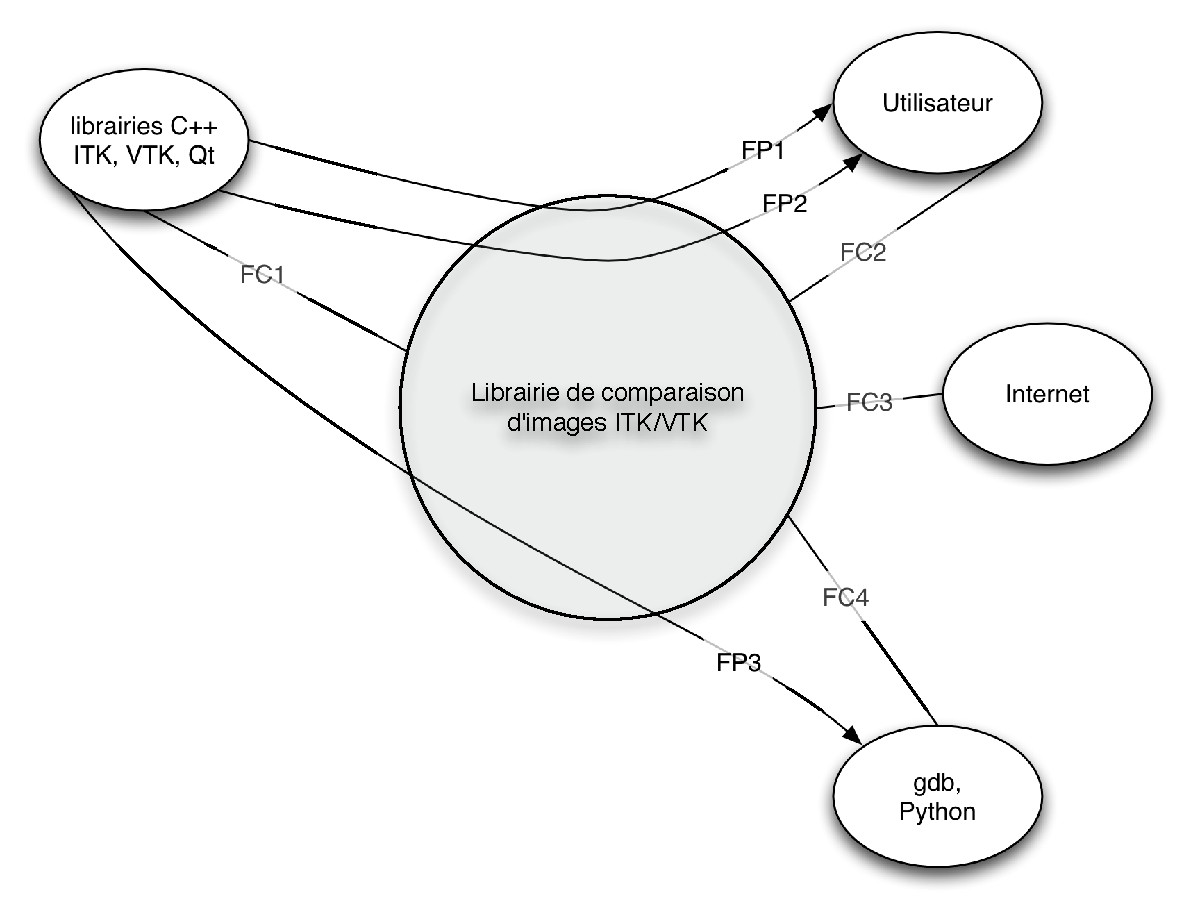
\includegraphics[width=0.95\textwidth]{pictures/ComparePIEUVRE}
\end{center}
\caption[Diagramme Pieuvre (méthode {APTE\textregistered}) de la librairie de comparaison d'images]{Diagramme Pieuvre (méthode {APTE\textregistered}) de la librairie de comparaison d'images
\small
\textbf{Fonction principale :}\\
FP1 : visualiser des données (fichiers ou en mémoire) provenant de VTK et ITK dans Qt\\
FP2 : synchroniser la visualisation de plusieurs images\\
FP3 : debugger visuellement des pipelines ITK et VTK dans gdb\\
\textbf{Fonctions contrainte :} \\
FC1 : être compatible avec VTK, ITK et Qt\\
FC2 : proposer une interface simple, une documentation, des exemples, et être facilement modifiable\\
FC3 : être visible sur internet\\
FC4 : être compatible avec Python pour interfacer avec gdb}
\label{fig:PIEUVRECompare}
\end{figure}

\paragraph*{FP1} : visualiser des données (fichiers ou en mémoire) provenant de VTK et ITK dans Qt
\begin{itemize}
  \item Existe pour afficher les résultats des traitements réalisés par des plugins ITK/VTK dans Gofigure2.
  \item Existe à cause de la complexité actuelle de l'utilisation d'ITK et VTK avec Qt. 
  \item Pourrait disparaitre si une librairie plus efficace et simple de visualisation était crée.
\end{itemize}

\paragraph*{FP2} : synchroniser la visualisation de plusieurs images
\begin{itemize}
  \item Existe pour comparer pixel(voxel) par pixel plusieurs images.
  \item Existe à cause du besoin des traiteurs d'image d'une telle comparaison.
  \item Pourrait évoluer si VTK ou le moteur 3D utilisé vtkINRIA3D\cite{vtkINRIA}
  proposaient des solutions simple de synchronisation de visualisations.
\end{itemize}

\paragraph*{FP3} : débugger visuellement des pipelines ITK et VTK dans gdb
\begin{itemize}
  \item Existe pour permettre au programmeur de rapidement visualiser des images a différents points d'une pipeline ITK ou VTK.
  \item Existe à cause du besoin de débugger les algorithmes de traitement d'image,
  et de visualiser les images d'une manière compréhensible par un humain.
  \item Pourrait évoluer si ITK, gdb ou Python évoluent.
\end{itemize}

\paragraph*{FC1} : être compatible avec VTK, ITK et Qt
\begin{itemize}
  \item Existe pour permettre a l'application de fonctionner.
  \item Existe à cause du fait que ces 3 librairies sont complémentaires et souvent utilisées conjointement dans une même application.
  \item Pourrait disparaitre si une librairie regroupant les fonctions d'ITK, VTK et Qt était crée, et si Gofigure2 l'utilisait.
\end{itemize}

\paragraph*{FC2} : Proposer une interface simple, une documentation, des exemples, et être facilement modifiable
\begin{itemize}
  \item Existe pour permettre a un utilisateur d'utiliser, comprendre et modifier la librairie.
  \item Existe à cause du fait qu'un code mélant ITK, VTK, et Qt n'est pas trivial.
  \item Pourrait évoluer avec la librairie.
\end{itemize}

\paragraph*{FC3} : être visible sur internet
\begin{itemize}
  \item Existe pour permettre a un maximum de programmeur de télécharger la librairie et l'utiliser.
  \item Existe à cause du fait que la librairie est open-source et s'améliore avec les contributions d'autres utilisateurs.
  \item Pourrait disparaitre si la librairie venait à ne plus être publique.
\end{itemize}

\paragraph*{FC3} : être compatible avec Python pour interfacer avec gdb
\begin{itemize}
  \item Existe pour permettre l'intégration à gdb et le débuggage b-visuel des pipelines ITK et VTK.
  \item Existe à cause du fait que gdb nécessite une interface python pour
  interpréter les données en provenance des pipelines ITKet VTK dans un programme externe.
  \item Pourrait disparaitre si gdb n'utilisait plus Python pour interfacer avec des programmes externes.
\end{itemize}

\subsection{les outils utilisés}
Afin de pouvoir programmer ce projet,il a été nécessaire d'apprendre à utiliser un certain nombre d'outils, de librairies et concepts {\C++}. Cet apprentissage a été une partie importante de mon PFE, me permettant d'acquérir de nouvelles compétences de valeur en sciences informatiques.
\subsubsection{Les librairies \C++}
Il existe un grand nombre de fonctions déjà codées en {\C++}.
Dans une optique de standardisation et d'efficacité, il est important d'apprendre
a utiliser des librairies contenant les fonctions utiles au programme que l'on crée.

Le projet utilise trois grandes librairies :
\begin{description}
  \item[Insight ToolKit (ITK)] qui est spécialisée dans le traitement d'image. Nous utilisons cette librairie, 
  afin de supporter le type de données qu'elle stocke en mémoire.
  \item[Visualization ToolKit (VTK)] qui est spécialisé dans la visualisation d'images. 
  Nous utilisons cette librairie afin de supporter le type de données qu'elle stocke en mémoire,
  et aussi pour visualiser les données acquises par la librairie.
  \item[Qt]\cite{refQT} qui est spécialisée dans la création d'interface graphiques. 
  Nous avons rendu notre travail directement compatible avec cette librairie
  pour permettre aux utilisateurs de l'intégrer dans n'importe quelle application développée avec Qt.
  \item[vtkINRIA3D]{\cite{vtkINRIA}} qui est le moteur 3D utilisé par Gofigure2\cite{refGofigure2},
  le programme développé au MegasonLab.
  Cette librairie permet d'explorer un volume tri-dimmensionnel en affichant trois coupes selon des plans perpendiculaires.
  Simultanément, un objet tridimensionnel composé par ces trois coupes est affiché.
  La version présente dans Gofigure2 à été grandement modifiée.
\end{description}
Une description détaillée de ces librairies est présentée en annexe.

\TODO{Annexe avec description pipelines etc... vtk itk qt}

\subsubsection{Les outils de programmation}
A partir d'un certain niveau, en {\C++}, il est indispensable de maitriser certains outils complexes. Ceux-la, après un temps
 d'apprentissage, augmentent grandement la productivité.
Les outils utilisés quotidiennement, dans le processus de développement d'applications au Megason lab sont :

\begin{description}
  \item[l'Unix Shell] : pratiquement tous les développeurs travaillent sur Linux car ce système inclut un grand nombre d'utilitaires
  standard pour un développement en {\C++}. Les outils de contrôle de version (SVN, GIT), les outils de connexion réseau (ssh), des
  compilateurs pour les principaux langages sont installes par défaut sur la plupart des distributions Linux.
  Afin de pouvoir bénéficier au maximum de ce système, il est important de maitriser l'invite de commande.
  \item[CMake] : ce programme permet de définir des règles de compilation pour différents compilateurs, afin qu'un projet puisse
   compiler sur différents systèmes d'exploitation (Nous programmons des application fonctionnant sur Windows, Linux et MacOs).
  \item[CTest] : Lorsque l'on travaille sur un projet volumineux, il est facile de "casser" le code. L'ajout de certaines fonctionnalités 
  peut modifier le comportement d'autres parties du programme d'une manière imprévue. L'outil CTest est utilisé au Kegason Lab, 
  pour tester la fiabilité du code. Ce programme télécharge régulièrement le code source, le compile, et effectue une batterie de test 
  des fonctionnalités du programme.
  \item[SVN] : Gofigure2 les développeurs de Gofigure2 travaillent sur les même fichiers simultanément. 
  Dans ce cadre, il est important de garder une trace des modifications apportées par chacun. Il faut aussi combiner ces changements, 
  et sauvegarder le projet sur un serveur accessible à tous. SVN est un programme de gestion de versions qui rempli toutes ces 
  fonctions.
\end{description}


\subsection{Agenda}

Afin de planifier les tâches accomplies pour mener à bien ce projet, un diagramme de Gantt est présenté.
\TODO{INSERER GANTT pour Comparer }

\subsection{Résultats et travail futur}

La librairie a été créée et est fonctionnelle. Elle rempli les fonctions présentées en introduction. Un exemple de code est donné en annexe, illustrant l'extrême simplicité d'utilisation de la librairie.
\TODO{insere code snapshot en annexe}
Une interface graphique basique a été crée pour illustrer les fonctionnalités de la librairie :
\TODO{include screenshots}
En plus d'un article dans l'Insight Journal, d'un code abondamment commenté, et d'une panoplie d'exemples,
la librairie est délivrée avec une documentation en ligne.
\TODO{inserer exemple documentation}
Afin de prouver la robustesse des classes utilisées, une série de tests automatiques a été crée.
La librairie a été intégrée au code de Gofigure2, au seins de se librairie graphique (QGoGUI), et est en ce moment intégrée au débugger graphique, en collaboration avec Matt MacCormick.

La librairie de comparaison d'images est un très bonne base à laquelle on peut ajouter de nombreuses fonctionnalités :
\begin{itemize}
  \item Supporter des images vectorielles d'ITK,
  \item intégrer des filtres simples (gradient, inverse, seuillage...),
  \item ajouter un moteur de rendu 3D (par tracé de rayons par exemple...).
\end{itemize}






%--------------------------------------------------
%             GIT
%--------------------------------------------------


\section{Définition d'un protocole de travail sous GIT}

Une partie de mon travail a consisté en la définition de protocoles 
afin d'effectuer certaines tâches d'une manière organisée et répétable. 
J'ai travaillé sur l'élaboration d'un protocole de travail sur GIT pour l'équipe de programmateurs.

Je suis donc passé par une phase de découverte et d'apprentissage pour ensuite écrire un tutoriel 
afin d'expliquer le fonctionnement de GIT a l'équipe informatique. 
J'ai ensuite propose un "workflow" utilisant GIT.

\subsubsection{Le contrôle de version}

Cette partie présente brièvement la gestion de version et les principales solutions existantes.

\paragraph{Le contrôle de version} ou gestion de version consiste en
la création d'un historique des modifications apportées a un projet.
Il est nécessaire de disposer d'un programme à cet effet,
surtout lorsque plusieurs personnes travaillent sur le même projet.
Il est ainsi possible de garder trace de toutes les modifications apportées.
Certains programmes de contrôle de version permettent
de modifier l'historique en annulant l'effet d'une modification erronée par exemple.

Les programmes récents de contrôle de version sont aussi utilisés
pour permettre a plusieurs développeurs de travailler 
sur le même fichier, ou sur des fonctionnalités différentes.

Il existe un vocabulaire particulier au contrôle de version.
Pour ce rapport, il est important de comprendre l'analogie de l'arbre couramment utilisée.
Le tronc (trunc) contient généralement la dernière version commune du projet.
De ce tronc, les programmeurs créent des branches pour apporter des changements.
Ces branches sont des copies du tronc.
L'action de sauvegarder dans l'historique les changements apportés au projet est "committer" (to commit).
L'action de fusionner une branche au tronc
(et ainsi rapporter tous les changements effectués sur une branche au tronc), s'appelle le merge.
Dans les  "anciens" programmes de gestion de version,
les changements (commits) sont souvent directement faits sur le tronc.
Cela crée des problèmes de conflits
(plusieurs utilisateurs auraient changé d'une manière différente le même fichier, par exemple).

Le code source est souvent stocké sur un serveur en ligne.
Ainsi, le programme de gestion de version est aussi utilisé
pour publier le code sur internet, par l'intermédiaire de sites spécialisés
(Sourceforge, Github, Gitorious, GoogleCode...).

\TODO{Illustration du fonctionnement d'un programme de gestion de version :}


\paragraph{Les deux philosophies de contrôle de version} sont actuellement la gestion de version centralisée et la gestion de version décentralisée. 
La gestion centralisée est basée sur un serveur qui contient la copie de référence des fichiers, 
et tout l'historique du projet. 
Les programmeurs n'ont sur leur ordinateur, que la dernière version du projet. 
Ce mode de fonctionnement nécessite une connexion au serveur pour faire avancer le projet.
La gestion décentralisée, par opposition, n'impose théoriquement pas de serveur central.
Les programmeurs disposent chacun d'une copie complète du projet sur leur ordinateur
qu'ils modifient a leur guise et synchronisent avec d'autres programmeurs.
Ce mode de fonctionnement permet de travailler sans connexion au serveur.

Il est possible de trouver une comparaison détaillée des deux philosophies à cette adresse :
\TODO{cite adresse \url{http://informatique.in2p3.fr/?q=node/333}}



\paragraph{principales solutions}

Il existe d'autres solutions :


SVN GIT Hg Bazaar...
presenter en annex comparaison.

wiki liste une trentaine de clients


\TODO{inserer un tableau avec les principaux clients, presenter comparaison en annexe}

\paragraph{Avantages de Git sur la concurrence}

GIT n'est pas le seul programme de contrôle de version. Son principal concurrent est Subversion.
Cependant il propose de nombreux avantages dont les principaux sont:
\begin{description}
  \item[rapidité] : GIT utilise un protocole de communication bien plus efficace que svn (a peu pres 5 fois plus rapide). 
  De plus, les commits peuvent être sauvegardes sans connexion au serveur central.
  \item[économie] : GIT utilise un algorithme de compression très performant : le code prend ainsi très peu de place.
  \item[développement en commun] : chacun peut travailler sur une sous partie du programme. La création de "branches" est facile et
  rapide. La mise en commun des changements est bien mieux gérée que sur des programmes concurrents comme SVN.
  \item[développement décentralisé] : chacun possède une copie du code et peut travailler sans connexion internet. 
  Si le serveur subit une panne ou est indisponible, tout le monde peut continuer à travailler, et la recréation d'un serveur est triviale.
  \item[Souplesse] : GIT permet de travailler sur un projet utilisant svn en bénéficiant des avantages de la gestion de projet
  décentralisée.
\end{description}


\subsection{Écriture du tutoriel}

Le tutoriel a été écris sur le wiki de Gofigure2. Il s'agit de l'emplacement de prédilection pour les informations 
concernant la programmation et l'utilisation de Gofigure2. Le système du wiki, en plus de proposer une syntaxe simple 
pour créer des pages web formatées, permet aux lecteurs autorisés de modifier le contenu. 
Il existe aussi un système de feedback permettant aux lecteurs ayant mal compris le contenu, de contacter l'auteur.

L'écriture d'un tel tutoriel se fait souvent dans un registre proche du langage familier,
le but étant de simuler des instruction données par un collègue ou un ami. 
Les instruction se doivent d'être relativement brèves, bien souvent le lecteur veut juste appliquer certaines fonctionnalités 
proposées par GIT sans toujours vraiment chercher a comprendre ce qu'il fait. 
Il existe d'autres sources d'informations pour apprendre complètement le fonctionnement de l'application.
Le tutoriel ne se veut donc pas exhaustif, il propose juste une manière qui fonctionne d'utiliser GIT,
a la manière d'un travail dirigé. Il a été écrit pendant ma phase d'apprentissage de GIT. 
Il détaille les principales difficultés et écueils rencontrés. 

Le tutoriel est présent a cette adresse : \\
\url{http://sourceforge.net/apps/trac/gofigure2/wiki/GIT}

\subsection{Proposition d'un protocole de travail}
Il a enfin fallu proposer un workflow (protocole de travail), qui définit la manière dont les programmeurs
doivent apporter des modifications au code source. Il s'agit de proposer un protocole qui :
\begin{enumerate}
  \item n'augmente pas trop la charge de travail,
  \item permette de bien suivre les modifications apportes par chacun. 
  \item permette au responsable du projet de corriger ou supprimer les changements apportes par les développeurs.
  \item corresponde a un standard.
\end{enumerate}
Le workflow proposé a été détaillé par \href{http://nvie.com/about }{Vincent Driessen} sur son \href{http://nvie.com/git-model}{blog}. Ce protocole découle assez naturellement de l'apprentissage de GIT, il est donc simple.

Ce workflow, en plus d'être précisément détaillé, est techniquement viable.

\subsubsection{description du protocole}

Il existe deux branches principales : 
\begin{description}
  \item[\emph{master}] : cette branche store les versions stables du programme.
  \item[\emph{develop}] : cette branche contient la dernière version commune du programme, elle correspond au tronc.
\end{description}
Ces branches sont présentes sur le serveur central. Le développement du programme se fait sur la branche \emph{develop}, et lorsqu'une version stable est sur le point d'être produite, on sauvegarde l'état d'avancement du projet dans la branche \emph{master}.

Il existe ensuite une série de branches de support.
Ces branches ont une durée de vie limitée, et doivent fusionner avec d'autres branches pour finalement rejoindre \emph{develop} (le tronc), puis \emph{master}.
Elles ne sont pas forcement présente sur le serveur central, cela dépend des équipes travaillant sur les différentes parties du programme.
\begin{description}
  \item[\emph{feature}] : cette branche contient le développement d'une fonction du programme. Elle est crée à partir de \emph{develop}, et une fois mature, refusionne avec \emph{develop}.
  \item[\emph{release}] : cette branche permet aux développeurs de travailler sur la correction de bugs, l'interface graphique, l'ajout de tests... les touches de dernière minute, avant la publication d'une nouvelle version du programme. Elle est crée lorsque la branche \emph{develop} contient toutes les fonctions attendues pour la nouvelle version du programme. Elle est créée à partir de la branche develop et une foi mature, fusionne avec la branche \emph{master}, et \emph{develop}.
  \item[\emph{hotfixes}] : cette branche particulière est créée à partir de la branche \emph{master}, lorsque une version publiée du programme contient un bug important qui ne peut attendre la prochaine version pour être corrigé. Elle refusionne avec la branche \emph{master} pour créer des "sous versions" (0.1.1 par exemple, est une sous version de 0.1.0). Cette branche particulière merge aussi avec la branche \emph{develop} pour appliquer la correction aux futures publications, et enfin, la branche \emph{release} si elle existe au moment de la réparation du bug.
\end{description}

Un cycle de développement simplifie devient donc, pour un programmeur :
\begin{figure}[H]
\begin{center}
\leavevmode
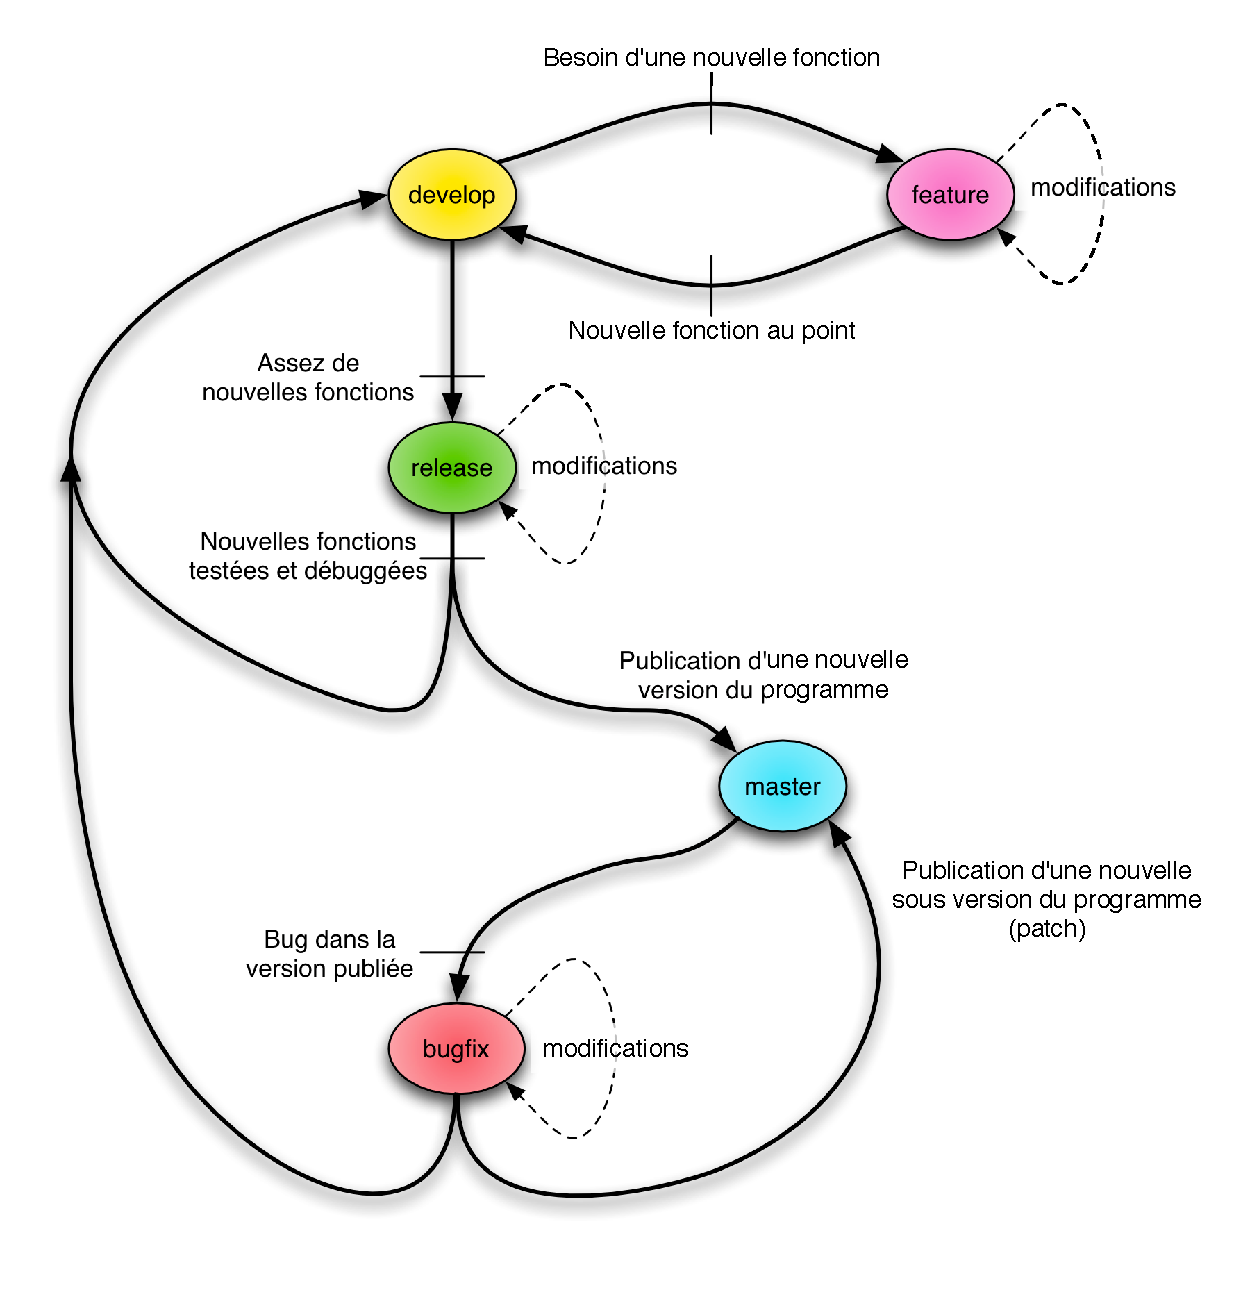
\includegraphics[width=0.95\textwidth]{pictures/GIT_WorkflowSimple}
\end{center}
\caption{Diagramme simplifié du workflow \\ proposé pour l'équipe de Gofigure2}
\label{fig:Workflow GIT de Gofigure2}
\end{figure}

Il est important de noter que bien souvent, les informaticiens travaillent sur plusieurs choses a la foi, et ce workflow permet ce genre d'organisation. 
Une illustration plus complete de ce protocole est présentée en annexe.
\TODO{insert workflow pdf ANNEXE}






%--------------------------------------------------
%             RECALAGE
%--------------------------------------------------

\section{Amélioration des techniques d'imagerie}



\subsection{Cahier des charges}
Le cahier des charges est présenté selon la méthode {APTE\textregistered}, Nous commençons donc par présenter la Bête à Cornes,
pour clarifier le but principal du projet. Nous présentons ensuite le diagramme pieuvre qui permet de clarifier les fonctions du projet.

\subsubsection{Contrôle de la validité du projet}
\begin{figure}[h]
\begin{center}
\leavevmode
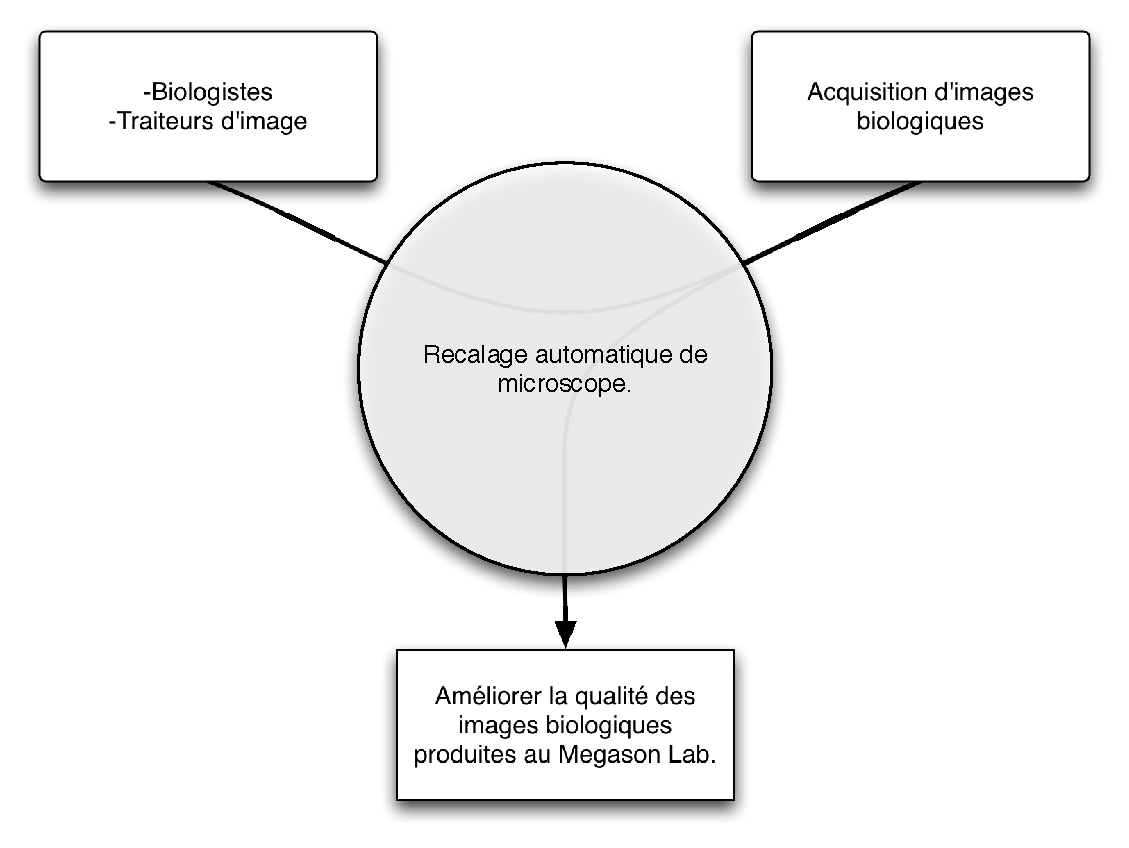
\includegraphics[width=0.95\textwidth]{pictures/RecalBAC}
\end{center}
\caption{Bête à corne (méthode {APTE\textregistered}) du projet de recalage}
\label{fig:BACRecal}
\end{figure}

La figure~\ref{fig:BACRecal} montre la Bête à Corne du projet de recalage d'images microscopiques.

Le but de ce produit résulte d'un besoin exprimé par les biologistes et traiteurs d'images.
Comme le spécimen change de forme durant le phase d'imagerie, il arrive qu'il ne soit plus dans le champ du microscope.
Cela est un réel problème pour les biologistes qui doivent contrôler l'alignement du microscope toutes les heures.
C'est aussi un problème pour les traiteurs d'image
car il arrive qu'un biologiste déplace en un mouvement un spécimen.
Cela invalide beaucoup de méthodes de suivi des objets imagés.

Ce projet, en automatisant l'alignement du microscope permet donc aux biologistes de moins surveiller l'acquisition,
et aux traiteurs d'images, de disposer de données exploitables.

Ce projet peut évoluer en accord avec les besoins des biologistes, et suivant l'évolution des techniques de recalage d'image.


\newpage
\subsubsection{Expression fonctionnelle}

\begin{figure}[H]
\begin{center}
%\leavevmode
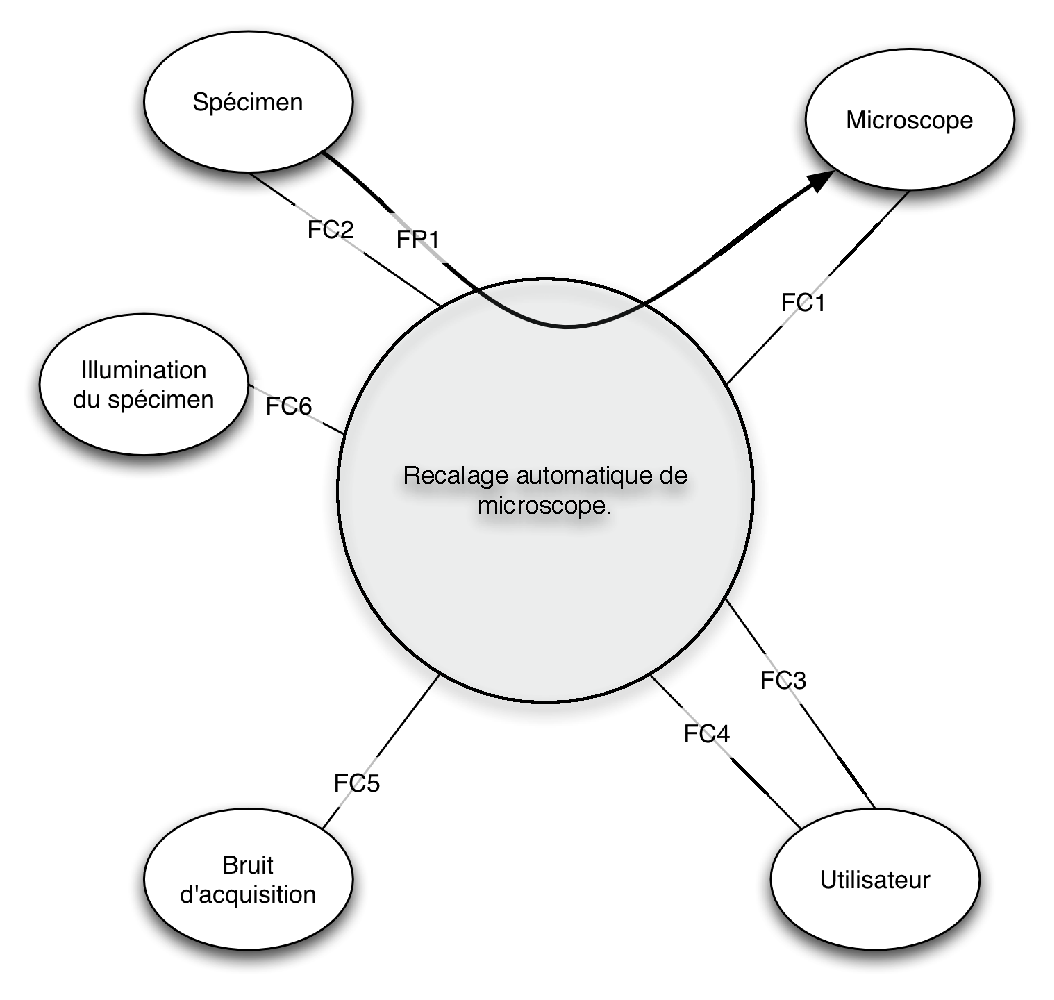
\includegraphics[width=0.9\textwidth]{pictures/RecalPIEUVRE}
\end{center}
\caption[Diagramme Pieuvre (méthode {APTE\textregistered}) du projet de recalage]{Diagramme Pieuvre (méthode {APTE\textregistered}) du projet de recalage
\small
\textbf{Fonction principale :}\\
FP1 : déplacer le microscope pendant l'acquisition en suivant le spécimen\\
\textbf{Fonctions contrainte :} \\
FC1 : compatible avec les logiciels utilises\\
FC2 : robuste aux changements de forme du spécimen\\
FC3 : contenir une interface homme machine\\
FC4 : maintenable par l'équipe du megason lab\\
FC5 : robuste au bruit\\
FC6 : robuste aux changement d'illumination}
\label{fig:PIEUVRERecal}
\end{figure}

La figure~\ref{fig:PIEUVRERecal} est le diagramme pieuvre du projet, que nous analysons :
\paragraph*{FP1} : déplacer le microscope pendant l'acquisition en suivant le spécimen.
\begin{itemize}
  \item Existe pour Créer des images exploitables d'une manière fiable.
  \item Existe à cause de la nature du spécimen analysé, qui est vivant et en développement. 
  Il change donc de forme, grossit et se déplace, il faut donc suivre l'organe d'interet pendant le
  développement du spécimen.
  \item Pourrait disparaitre si le Megason Lab arrêtait d'imager des spécimens vivants.
  Si les microscope avaient un champ de visualisation assez grand pour englober
  tout le spécimen et d'éventuelles marges de déplacement.
\end{itemize}

\paragraph*{FC1} : compatible avec les logiciels utilises.
\begin{itemize}
  \item Existe pour fonctionner avec le matériel présent au Megason Lab.
  \item Existe à cause de la nature des logiciels utilisés au Megason Lab.
  \item Pourrait disparaitre si le logiciel de contrôle du Megason Lab était compatible avec n'importe quel langage informatique,
  en particulier le {\C++}.
\end{itemize}

\paragraph*{FC2} : robuste aux changements de forme du spécimen
\begin{itemize}
  \item Existe pour fonctionner sur différents spécimens analysés.
  et fonctionner sur une période de temps étendue (le spécimen change de forme au cours du temps).
  \item Existe à cause de la nature des spécimens analysés au Megason Lab.
  \item Pourrait disparaitre si les spécimens n'évoluaient pas au cours du temps;
  si il existait un programme spécifique à chaque partie du spécimen.
\end{itemize}

\paragraph*{FC3} : contenir une interface homme machine
\begin{itemize}
  \item Existe pour interagir avec l'utilisateur.
  \item Existe à cause du besoin du programme de paramètres provenant de l'utilisateur.
  \item Pourrait disparaitre si le programme pouvait déterminer automatiquement les meilleurs paramètres.
\end{itemize}

\paragraph*{FC4} : maintenable par l'équipe du megason lab
\begin{itemize}
  \item Existe pour permettre aux autres chercheurs du Megason Lab de modifier/utiliser le programme
  \item Existe à cause du fait que le développeur de l'application ne sera pas toujours présent pour la maintenir.
  \item Pourrait disparaitre si le programme se maintenait tout seul.
\end{itemize}

\paragraph*{FC5} : robuste au bruit
\begin{itemize}
  \item Existe pour permettre a l'algorithme de fonctionner en la présence de bruit
  \item Existe à cause du fait que le microscope produit des images bruitées.
  \item Pourrait disparaitre si le microscope produisait des images sans aucun bruit.
\end{itemize}


\paragraph*{FC6} : robuste aux changement d'illumination
\begin{itemize}
  \item Existe pour permettre a l'algorithme de fonctionner au cours du temps. 
  \item Existe à cause du fait que la fluorescence des spécimens décroit au cours du temps (phénomène de "bleaching"),
  et change d'une image à l'autre constante car le système d'illumination basé sur une probabilité d'absorption de photons
  (le même phosphore n'absorbe pas toujours autant de photons avant de ré-émettre).
  \item Pourrait disparaitre si le bleaching disparaissait 
  et si nous contrôlions mieux l'absorption de photons par les phosphores du spécimen.
\end{itemize}

\subsection{Solutions techniques}

Le principe du programme est d'estimer le déplacement de structures notables dans l'image.
Une fois ce déplacement estimé, il s'agit de déplacer le spécimen afin de garder ces structures dans le champ du microscope.

\subsubsection{Estimation du déplacement du spécimen}
Nous utilisons une technique connue sous le nom de recalage d'image pour estimer le déplacement du spécimen entre deux acquisitions (deux images) effectuées par le microscope.
Comme le microscope ne peut que déplacer le spécimen en translation, nous choisissons un recalage rigide qui évalue les translations selon les trois dimensions de l'espace, entre deux images.

Ces techniques sont basés sur des critères d'énergies à minimiser.
On choisit ces énergies de manière à ce que leur valeur soit élevée quand deux images sont mal alignées,
et faibles quand elles sont alignées. Notre programme teste différentes translations jusqu'à trouver une translation
qui donne une faible valeur du critère d'énergie.
Bien sûr, il n'est pas possible de calculer le critère d'énergie pour toute les translations possibles.
On choisit donc une technique qui "dirige" les estimations de manière à diminuer l'énergie (la descente de gradient est une technique classique).
Enfin, afin que notre algorithme soit robuste vis à vis du bruit, et des changements de forme peu significatifs,
nous moyennons les images, puis réduisons la résolution des images moyennées. Le facteur de reéduction dépend de la taille du spécimen, des structures à analyser, et de la résolution initiale des images acquises par le microscope.



\subsubsection{Stabilisation de l'acquisition}

\paragraph{Principe}


demarche : evaluation de la metrique
optimisation tps calcul
developpement en visualbasic (windows emule)


\subsubsection{Integration au microscope}



\subsubsection{Code}



\subsubsection{Tests et travaux futurs}
test sur objet inanime
test sur poisson en developpement
developpements futurs :
metrique non rigide ?
tps de calcul ?
wavelets pour downsample ?


\subsection{Agenda}





\subsection{Resultat}





\section{Conclusion de la partie ingénierie du PFE}


\section{Projet professionnel}

Ce PFE s'inscrit dans un projet professionnel construit durant ma scolarité a l'INSA de Lyon.
Mon inscription a l'INSa de Lyon a été grandement motivée par l'ouverture de l'école a l'international. J'ai ainsi effectue mon stage ouvrier en Afrique du Sud. Profitant d'une première expérience professionnelle a l'international.

Lors de ma seconde année a l'INSA de Lyon, j'ai choisi l'option SCiences et ANglais (SCAN). Cette filière regroupe les élèves ayant un niveau suffisant pour pouvoir suivre la formation généraliste en anglais. Elle s'accompagne d'une bourse pour un bref séjour linguistique dans une université étrangère. J'ai profite de ce financement pour aller au Trinity College en Irelande ou j'ai pu avoir ma première expérience académique a l'étranger.

J'ai ensuite choisi le département Génie Électrique qui permet de bénéficier d'un grand panel de compétences, notamment dans des domaines rattaches a l'électronique et l'informatique.

Continuant l'expérience internationale, j'ai effectué mon stage industriel au Fraunhofer Institute, Center for Manufacturing Innovation, aux États Unis. Ce stage m'a énormément apporte en plus de l'expérience technique. Il s'agissait d'une première immersion dans la culture américaine. C'est après ce stage que j'ai passe le test TOEIC validant un très bon niveau d'expression et de compréhension en anglais, avec un score de neuf cent quatre-vingt sur neuf cent quatre-vingt dix.

Le PFE au Megason lab possède des attraits indéniables : il s'agit d'un stage de recherche perfectionnant mes connaissances en traitement de l'image. Il s'agit aussi d'une expérience internationale dans une université renommée : Harvard Medical School. Ainsi, en plus de prendre plaisir a travailler en recherche, j'ouvre la porte a de nombreuses opportunités professionnelles.

Comme je suis intéressé par les domaines techniques, je compte profiter de l'opportunité de poursuivre mes études pour obtenir un doctorat en mathématiques appliquées, au cours d'une thèse élaborée en collaboration avec le laboratoire CREATIS (INSA Lyon) et le laboratoire Megason (Harvard Medical School). Cette incroyable opportunité professionnelle est financée en partie par Harvard Medical School et en partie par l'INSA de Lyon. Je passerai ainsi la moitié de mon temps en France, et l'autre moitie aux États Unis.
En plus de pouvoir travailler sur un domaine passionnant, je pourrai ainsi bénéficier d'une équivalence avec un PhD () (diplôme très reconnu a l'international). 

Je compte ensuite mettre en valeur ma capacité a travailler dans un contexte international, dans des domaine a haute technicité pour travailler dans le secteur privé. Je pourrai mettre en avant mes capacités en traitement du signal pour travailler dans le médical ou l'aéronautique.

Mon ambition est de migrer vers des responsabilités manageriales après avoir une très bonne maitrise de la technique.





\appendix


\chapter{Librairies utilisées pour le projet de Comparaison d'images}


\paragraph{La librairie "Insight ToolKit" (ITK)} est un projet open source initialement destiné au recalage et a la segmentation d'images medicales. ITK a été programmée en \C++ , en utilisant des techniques de codage avancées (templates, modification de la syntaxe standard et ajout de fonctionnalités au langage \C++ par le biais d'idiomes) , ainsi que l'outil de développement cross-platform CMake, et communautaires (SVN, puis GIT). 
Cette librairies est construite sur un système de "Templates", qui lui permet de s'adapter à diverses données. Elle propose une architecture centrées sur un flux de données, traité par différents filtres que l'on connecte ensemble.
Cette collection d'algorithmes ne cesse de s'agrandir grâce à la philosophie open-source. Le spectre des applications d'ITK inclut entre autres exemples:  
\begin{itemize}
  \item l'imagerie medicale, avec \href{http://www.slicer.org/}{3DSlicer},
  \item l'imagerie biologique, avec \href{http://gofigure2.sourceforge.net/}{Gofigure2},
  \item et l'imagerie satellite, avec l'\href{http://www.orfeo-toolbox.org/otb/}{Orfeo ToolBox}.
\end{itemize}
Le modèle de programmation est relativement complexe et nécessite de un long apprentissage, et de l'expérience. A cette fin, de nombreux outils d'information sont mis a la disponibilité du nouvel utilisateur :
\begin{itemize}
  \item des listes de diffusions d'Emails, pour mettre en contact les nouveaux utilisateurs d'ITK et les programmeurs et utilisateurs avancés;
  \item un wiki (\url{http://www.vtk.org/Wiki/ITK}), qui donne quelques informations quand à la mise en place d'un environnement de développement utilisant ITK.;
  \item un guide d'utilisateur très bien expliqué, mais basé sur la version 2.4 d'ITK tandis que la dernière version publiée est la 3.20;
    \TODO {reference ITK software guide}
  \item la documentation Doxygen présentée sous forme de site internet, est directement compilée a partir du code source. Elle est donc plus ou moins complète selon les fichiers. Afin de pouvoir naviguer dans cette dernière, il est indispensable de connaitre la structure du projet.
\end{itemize}
Luis Ibáñez, a dit cette année : "La courbe d'apprentissage d'ITK en \C++ est bien trop raide, et nous allons nous efforcer dans les futures version, de rendre la librairie plus accessible.". La prochaine version d'ITK (version 4) sera donc surement plus facile a utiliser et prendre en main.

\paragraph{La librairie VTK} est développée par Kitware, Il s'agit d'une librairie \C++ utilisee pour la visualisation de données. Elle est open source et cross-platform. Elle utilise des outils similaires a ceux utilises pour ITK (CMake)
Elle utilise un systeme de "pipeline" (flux de donnees) similaire a celui d'ITK pour traiter les donnees a visualiser. Elle est developpee conjointement avec ITK, et il est possible plus ou moins facilement de connecter les filtres de traitement d'image d'ITK avec les filtres de visualisation de VTK.

\paragraph{La librairie Qt} permet une gestion avancée de l'interface utilisateur, en proposant une interface graphique open source et cross-platform.
Elle étend aussi les fonctionnalités du langage \C++ en proposant une nouvelle architecture pour le système de callbacks, un nouveau modèle d'objet, et d'héritage. Cependant, ces modifications sont facilement intégrées par le développeur débutant, grâce a une aide abondante composée d'un ensemble de tutoriels, d'exemples fortement documentes, et d'une liste de diffusion très active.







\chapter{Définitions}




Templates : En programmation informatique, les templates sont une particularité de la programmation en language C++, qui autorise l'écriture d'un code sans considération envers le type des données avec lesquelles il sera finalement utilisé. Les templates supportent la programmation générique en {\C++}.

Cross-platform : Un logiciel multiplate-forme ou multiplateforme est un logiciel conçu pour fonctionner sur plusieurs plates-formes, c’est-à-dire le couple liant ordinateur et système d’exploitation. En anglais on parle souvent de "cross-platform software" ou "platform independent software" ou encore de "multi-platform software".

Idiomes (programmation) :  Un idiome en programmation qualifie un code qui ajoute des fonctionnalités non existantes dans un
langage.

Wiki : Un wiki est un site web dont les pages sont modifiables par tout ou partie des visiteurs du site. Il permet ainsi l'écriture et l'illustration collaboratives de documents.

Graphical User Interface (GUI) : Un environnement graphique est, en informatique, ce qui est affiché en pixels sur un moniteur
d'ordinateur et sur lequel l'utilisateur peut agir avec différents périphériques d'entrée comme le clavier ou la souris. 
Des images, des animations (en 2 ou 3 dimensions), et même des vidéos peuvent être rendues à l'écran.
Ce type d'interface Homme-machine s'oppose à la notion de ligne de commande.

Callback : la technique des fonctions de rappel (callback functions) permet de passer en argument d'une fonction, une autre fonction. 
Cette technique est utilisée dans la programmation évènementielle, ou les interactions de l'utilisateur doivent entrainer l'exécution de fonctions.

\chapter{Biblio TODO}

Evaluation/comparaisons de GIT :
descritpion comparaison centralisee non centralisee
\url{http://informatique.in2p3.fr/?q=node/333}
avantages de GIT :
\url{http://www.whygitisbetterthanx.com/}
\url{http://joshcarter.com/productivity/svn_hg_git_for_home_directory}
\url{http://dev-heaven.net/wiki/20/Git_vs_SVN_comparison}

Matt Mc Cornick

